\section*{Exercice 162 -- Schéma cinématique}

\setcounter{exo}{0}

Soit le système suivant. 

\begin{center}
 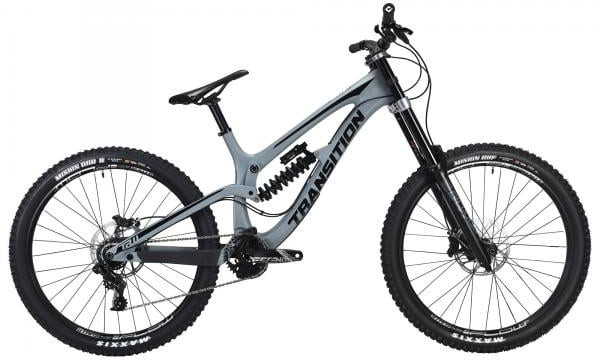
\includegraphics[width=.47\linewidth]{056_01}
 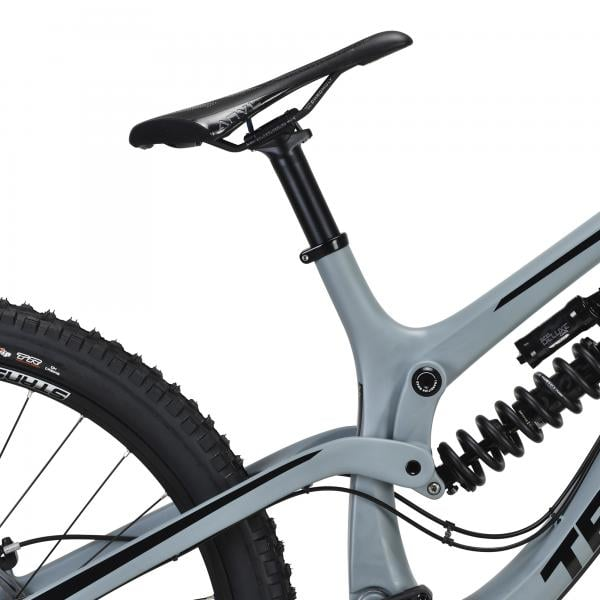
\includegraphics[width=.47\linewidth]{056_02}
\end{center}

\begin{center}
 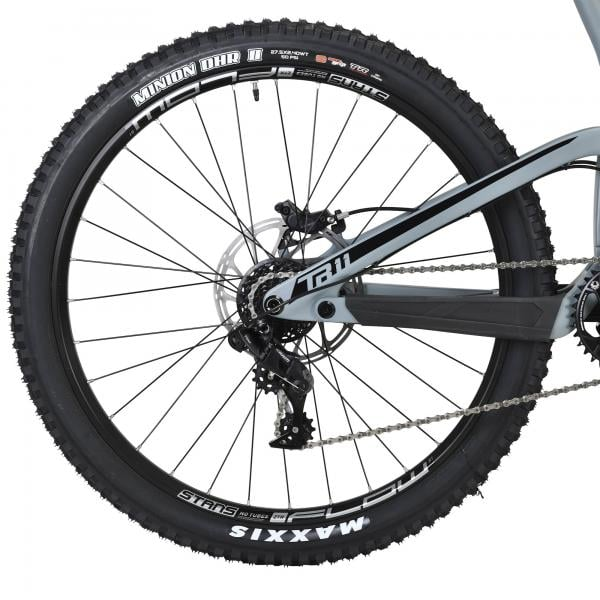
\includegraphics[width=.47\linewidth]{056_03}
 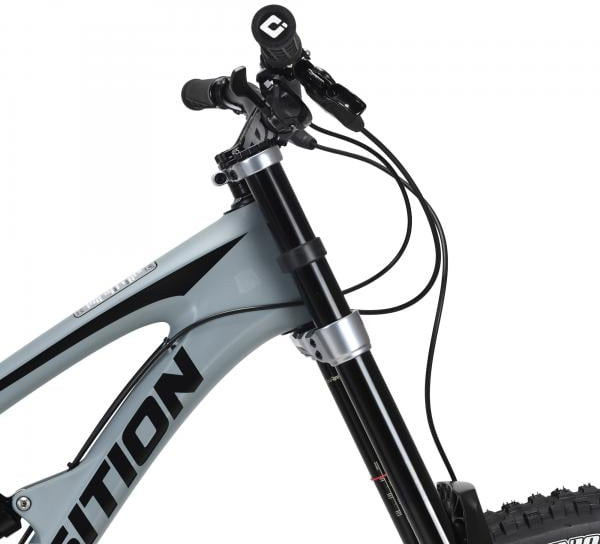
\includegraphics[width=.47\linewidth]{056_04}
\end{center}



\subparagraph{}
\textit{Proposer un schéma cinématique.}
 \ifprof
 \begin{corrige}
 
 \end{corrige}
 \else
 \fi

